\section{Verification} \label{s:N_II:validation}


This part of the chapter contains different comparisons and network metrics analyses to test and validate the changes made to the network pipeline. Changes in graphs between a tumour and non-tumour network are presented in \cref{s:N_II:net_comp}, the difference in the two reward functions is presented in \cref{s:N_II:reward_comp}, and the effects of the integrative MEV introduced to MIBC subtypes are covered in \cref{s:N_II:mev_comp}. The difference in the community detection algorithms is not covered as the \acrlong{hsbm} is a nested SBM that allows us to discover more communities than the standard SBM; the comparison between Leiden and SBM was covered in \cref{s:N_II:rwd}.


% Network validation 
\subsection{Healthy vs Tumour Network} \label{s:N_II:net_comp}

To study the differences between the non-tumour and tumour networks, the previously used graph metrics (degree, pageRank, closeness, betweenness and IVI)\footnote{Reminder: the degree - node's number of connections; pageRank - node's centrality;  closeness - how close the nodes are; betweenness - nodes between; IVI - a combination of network metrics} are shown in \cref{fig:N_II:net_metrics_comp}. There are four networks compared:
\begin{enumerate}
    \item \textbf{Tumour standard \& reward} - networks derived from tumour dataset with or without mutation burden integration (mustard \& red)
    \item \textbf{Healthy reward \& standard} - network derived using the non-tumour dataset with or without mutation burden integration (blue, green)
\end{enumerate}


% Degreee & PageRank
\subsubsection*{Degree \& PageRank}

For the non-tumour derived networks, there appears to be a subset of nodes that are highly connected, as indicated by the third quartile (Q3 - 5.47) being 60\% higher than the median degree value (3.36); see degree plot top left. The reward modifier seems to further promote these nodes, with the Q3 value remaining similar ($\sim$5.98), while the maximum degree increases 25 times, shifting the distribution towards a more pronounced long tail. This is a significant difference between the non-tumour reward and the standard network (\acrshort{mw}: 6250347.0,p-value: 0.0), and with the tumour networks (\acrshort{kw}: 682.7330180938997,p-value: $5.577e^{-149}$); shown in \cref{fig:N_II:net_metric_sig_std}.

A similar trend is observed in the PageRank metric, although the median score decreases by nearly a third (from $161$ to $105$) in the reward network, which may suggest that highly connected nodes are linked to less influential vertices. In contrast, TCGA-derived graphs show nodes with similar centrality and degree values, exhibiting less pronounced skewness at the top. The differences are significant between the two non-tumour networks (\acrshort{mw}: 21010334.0.0,p-value: 0.0), and with a healthy reward network compared to tumour networks (\acrshort{kw}: 2296.1121,p-value: 0)

\begin{figure}[!htb]    
    \centering
    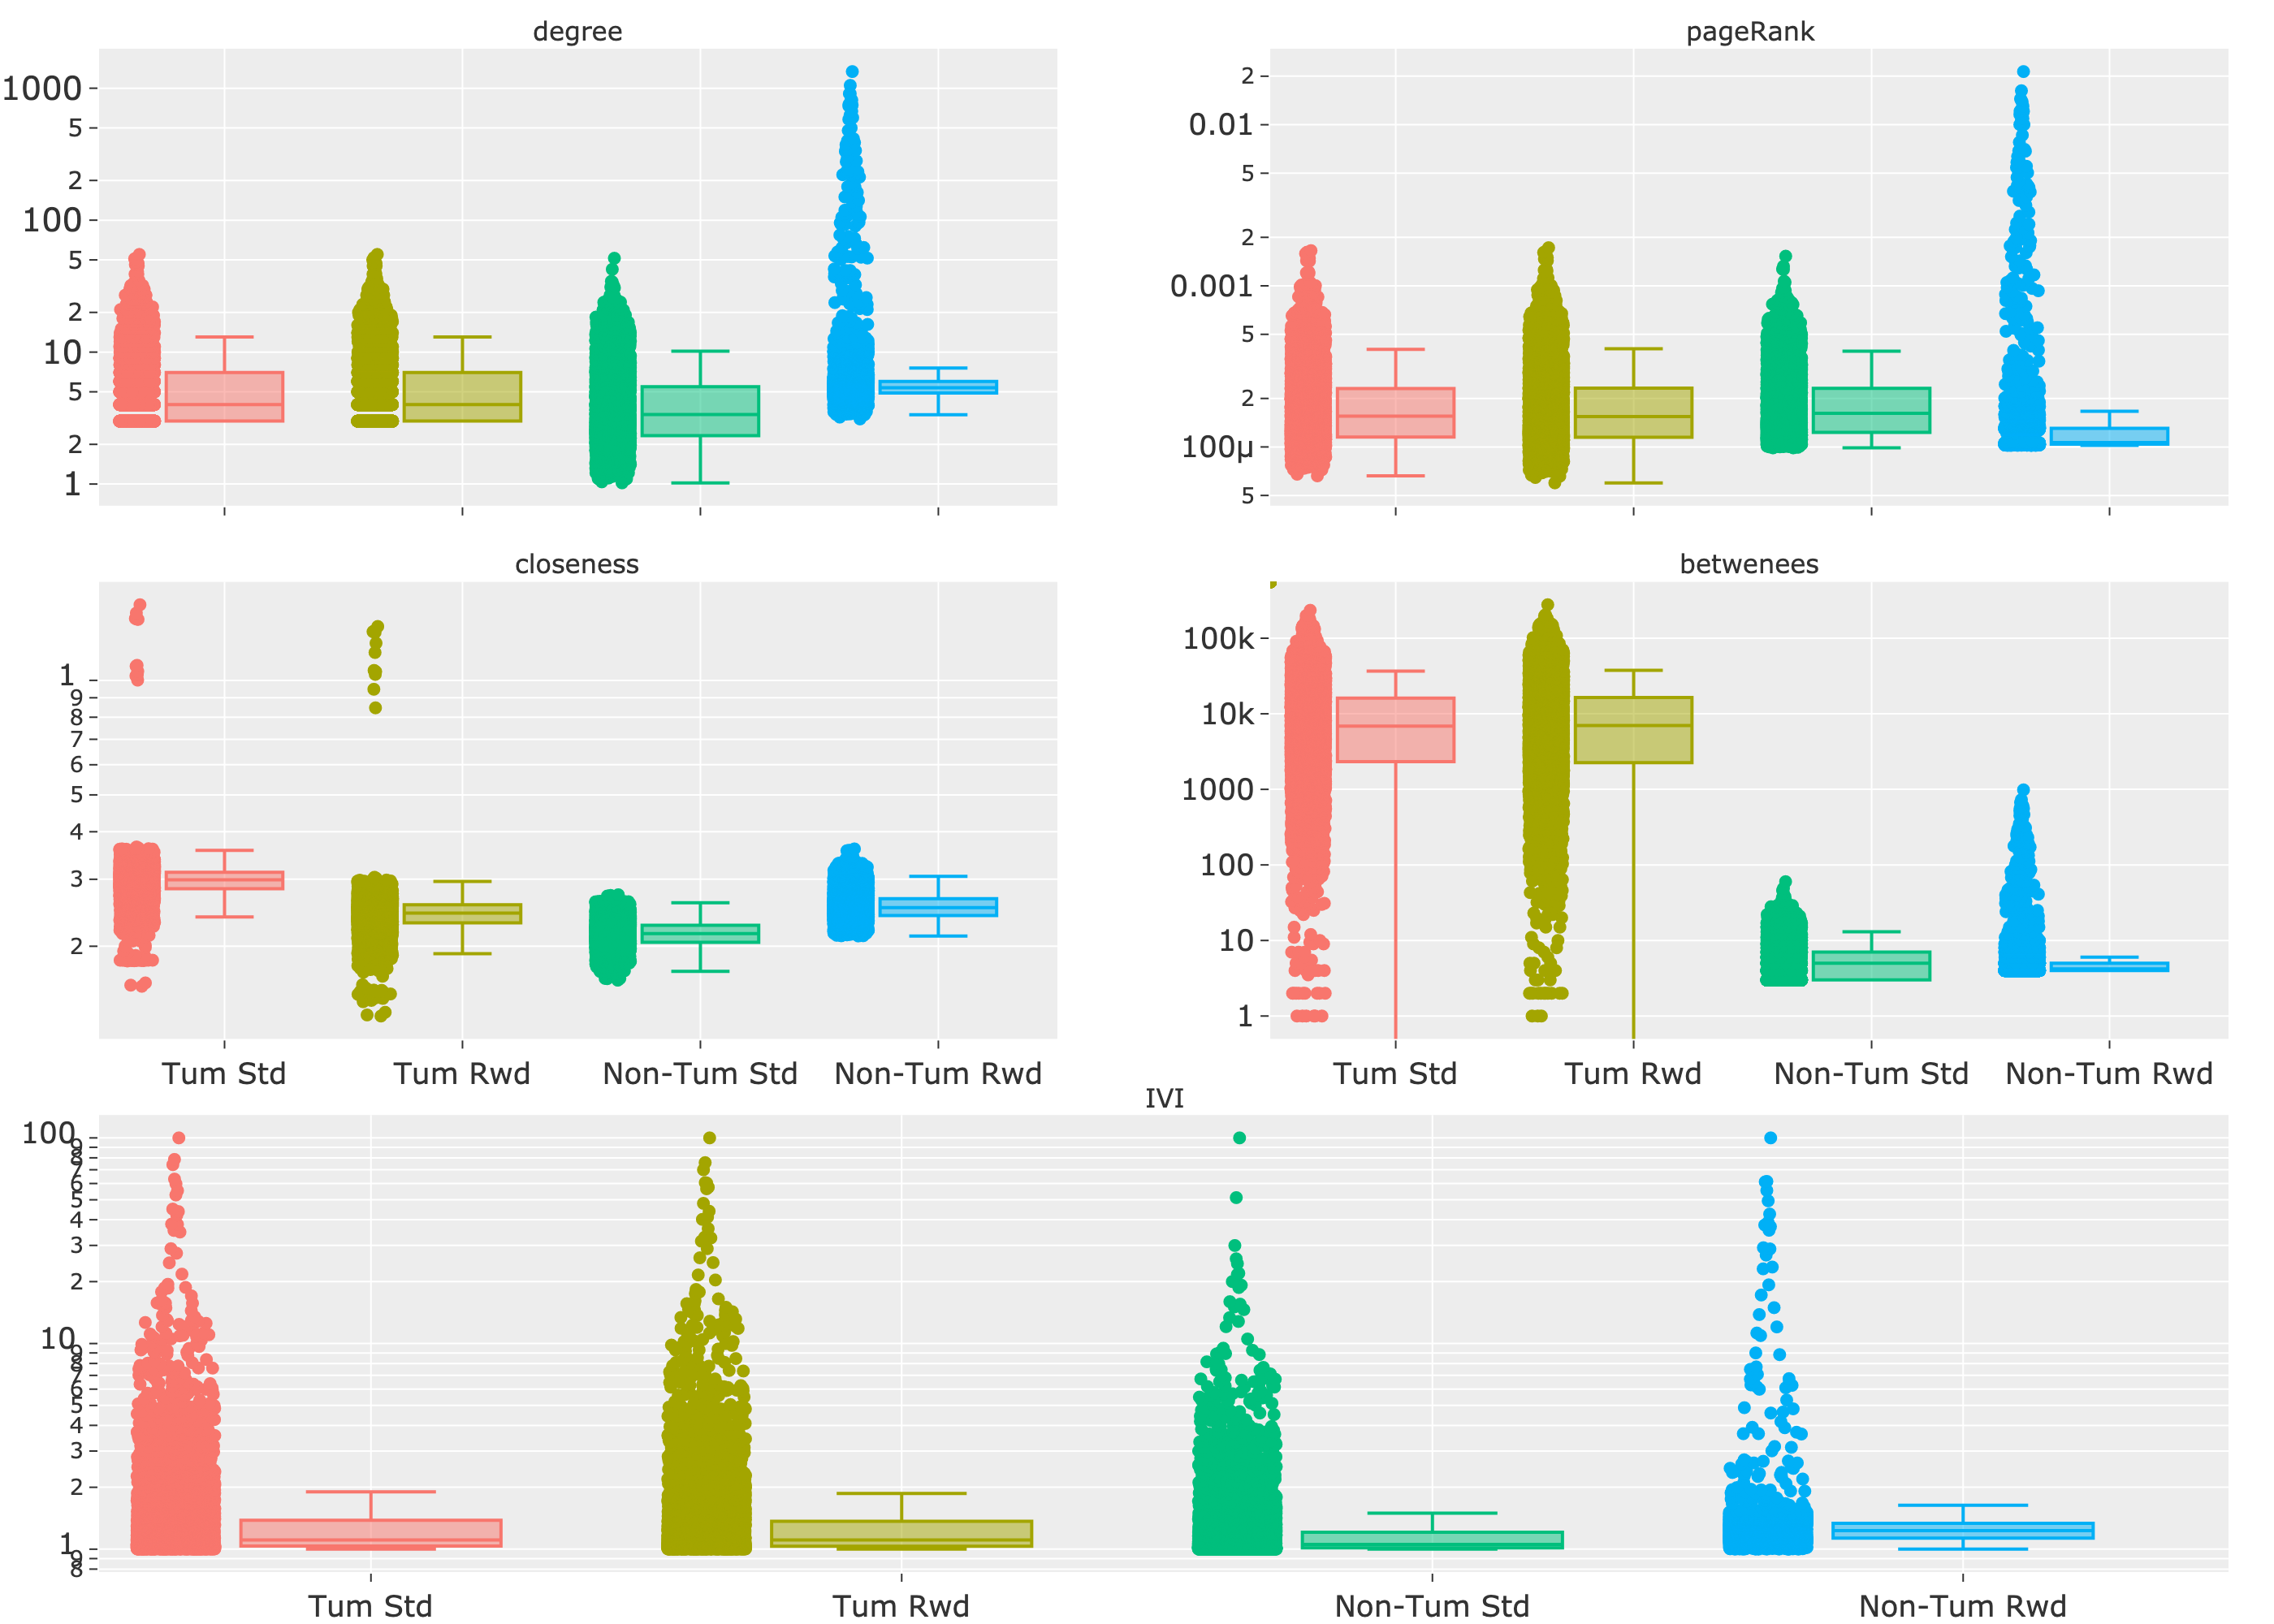
\includegraphics[width=1.0\textwidth,keepaspectratio]{Sections/Network_II/validation/network_comparison.png}
    \caption[Network metrics for cancerous and healthy graphs]{Network metrics for the Tumour and non-tumour networks with no modifier and reward modifier. The y-axis represent the log10 of the metric, see \cref{s:lit:net_metrics} for a description of the metrics. The y-axis represent is in log scale of the metric. Higher the degree and pageRank values more important the node is to the network, smaller values of closeness metric indicates that the vertices are closer together, while higher values of betweenness means that a node serves as a key bridge between other nodes. Higher values of \acrlong{ivi} indicates the node has a large influence both locally and globally to the network. The metrics comparisons shows that the non-tumour network react strong to the sigmoid modifier compared to the tumour derived graphs. There is also a subset of genes that are more central and have a large number of connections.}
    \label{fig:N_II:net_metrics_comp}
\end{figure}


% Closeness & betweneess
\subsubsection*{Closeness \& betweenness}

The reward modifier has significantly distinct effects on the two network types (\acrshort{kw}: 13078.435,p-value: 0.0), for the non-tumour graphs, it divides the nodes apart with a mean closeness (0.244) decreasing\footnote{Reminder: for closeness lower values are the better} by $\sim$20\% over the standard network (mean 0.298); the two distributions are significantly different (\acrshort{mw}: 1480750.0,p value: 0.0). The opposite effect occurs for tumour networks where, in general, the mean closeness values increase by $\sim$14\% from standard to reward network\footnote{Mean standard 0.216, reward 0.252} (\acrshort{mw}: 23670821.0,p-value: 0.0).

% This is given 
In addition, a decrease of $20$\% in betweenness metric across the non-tumour graphs indicates that there are fewer nodes as key connection points, but a few vertices are the important bridge. This is given by the higher variance in the metric for standard compared to the reward network, which has an almost flat box with a few outliers in q3. This behaviour is not seen in the two tumour networks, where the two distributions have a similar shape.

% IVI
The IVI distributions for the two tumour networks are not significantly different (\acrshort{mw}: 12532555.0,p-value: 0.821), but there is a noticeable difference between the non-tumour standard and reward networks (\acrshort{mw}: 6702904.0,p-value: 0). In the latter, the IVI distribution is elongating towards higher values, indicating that a subset of genes gained higher influence in the network, while the other's importance is lowered.


The edge weight modifier has two distinct effects on the networks. In tumour-derived graphs, the distributions are less impacted, and the nodes tend to cluster closer together, an effect that was observed in \cref{s:N_I}, \cref{fig:N_I:mut_rep_tum}. In contrast, for the non-tumour networks, a subset of genes gains a significant number of connections, and the nodes generally spread further apart after integrating the mutation burden. Vertices with a higher degree are explored in more detail in \cref{s:N_II:high_conn}. These trends might be explained by the presence of an existing signal in the tumour expression of the genes, which is only amplified by the integration of the mutation burden. In the non-tumour networks, however, this signal is absent, and integrating the mutation burden might reveal disruptions in normal cellular functioning.

\subsubsection*{Comparing with P0 derived networks}

In the analysis of freshly isolated cells (P0) from \cref{s:N_I:p0_tum_description}, a subset of highly connected nodes was observed, similar to the findings in this chapter. However, the first iteration of the weight modifier does not notably affect the centrality metrics, as the sigmoid modifier does. Additionally, in the P0 network, the reward network nodes were closer together than the standard and not further spread apart as in the non-tumour graphs.

The differences may be attributed to the additional datasets in the non-tumour network (gene expression from ABS-Ca and UD samples) and the changes in the genes used for the network construction. Although the overall closeness scores have similar median values across both network types, the outliers observed in the P0-derived graphs are absent in the non-tumour networks.


% Reward 1 vs Reward v2
\subsection{Comparison between reward functions} \label{s:N_II:reward_comp}

% Do I need the following two paragraphs?
A sigmoid function is used as a reward modifier for the improved network pipeline presented in this chapter. The differences in how the weights are changed by the two functions are shown in \cref{s:N_II:reward}. The networks effects of the two reward functions on the network is studied in this section.

In the previous sections, the network differences between the standard and modified networks were studied through the bar plots. The comparisons involved three networks as three histograms on a single plot resulted in cluttered figures. In this section, only the standard and the reward with the sigmoid function are compared over the usual clustering metrics utilised in this PhD project, as well as the Katz Centrality metrics; see \cref{s:lit:net_metrics} for more information.


% Talk about the stats and the difference between the stats
\begin{figure}[!b]    
    \centering
    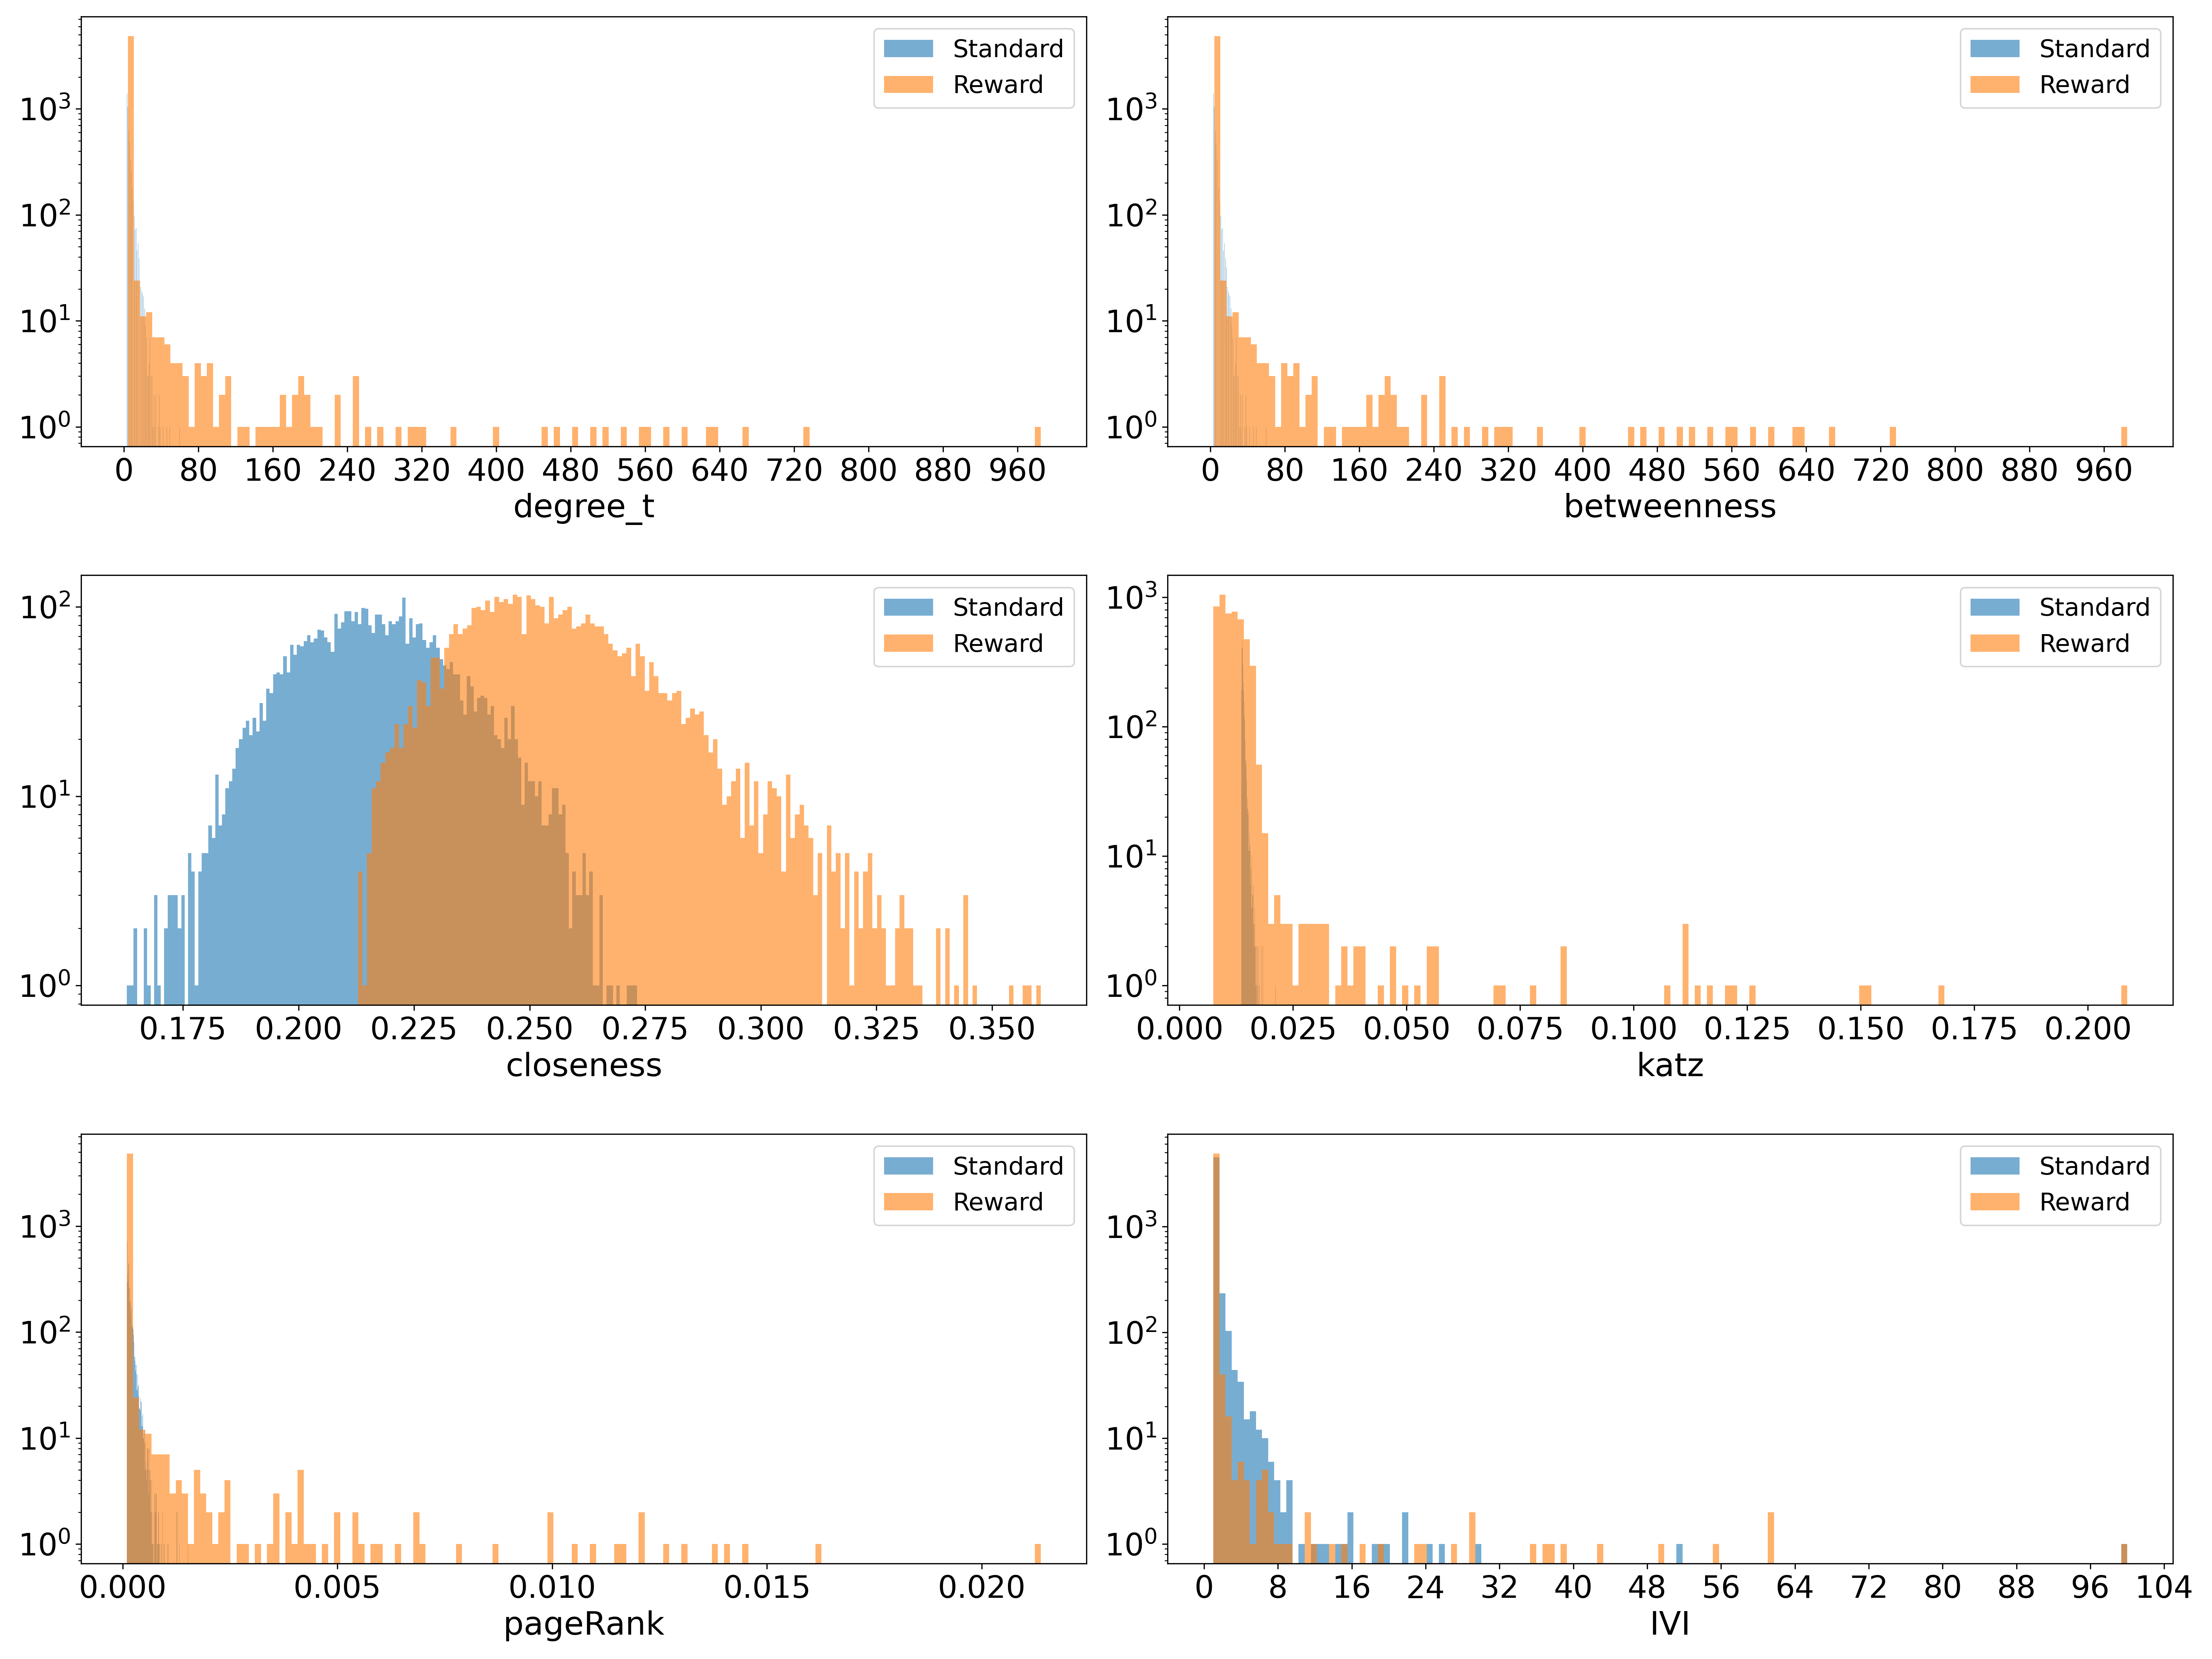
\includegraphics[width=1.0\textwidth,height=1.0\textheight,keepaspectratio]{Sections/Network_II/validation/net_metrics_Standard_Reward.png}
    \caption[Network metrics for healthy graphs]{Distribution of the network metrics for non-tumour standard and reward networks: total degree (degree\_t), betweenness, closeness, katz centrality, pageRank and IVI.  Higher the degree and pageRank values more important the network is to the network, smaller values of closeness metric indicates that the vertices are closer together, higher values of betweenness means that a node serves as a key bridge between other nodes. Higher values of \acrlong{ivi} indicates the node has a large influence both locally and globally to the network. The distributions showed that integrating the mutation burden into the networks alter nodes attributes to have a more pronounced long-tail distribution. It also highlights that there are a number of genes which have very high scores across  all network metrics.}
    \label{fig:N_II:net_metric_sig_std}
\end{figure}

% Analyse the metrics
The six metrics are shown in \cref{fig:N_II:net_metric_sig_std}, where the x-axes represent the graph metrics and the y-axes the log10 count. The orange bars correspond to the reward network and the blue bars to the standard network. Across the six plots, there is a significant difference between the standard and reward-modified networks; see \cref{tab:N_II:standard_vs_reward}. In the reward network, the nodes' attributes exhibit right-skewed distributions. This indicates that, in the standard graph, the nodes have relatively similar importance and proximity within the network, whereas in the reward network, a small subset of genes becomes highly connected and central. The distribution of the closeness metric suggests that nodes in the standard network are clustered more tightly together compared to those in the reward network. These metrics demonstrate that integrating the mutation burden results in a network with pronounced long-tail distributions of the node centrality metrics.

\begin{table}[!htb]
  \centering
  \small
  \begin{tabularx}{\textwidth}{>{\hsize=.5\hsize}X|>{\hsize=.5\hsize}X|>{\hsize=.5\hsize}X}
    \toprule
    \textbf{Metric} & \textbf{MW} & \textbf{p-value} \\
    \midrule
    \textbf{Betweenness} & 1126503.5 & 0.0 \\
    \midrule
    \textbf{Closeness} & 3951965.0 & 0.0 \\
    \midrule
    \textbf{Degree} & 8543780.5 & $2.999e^{-166}$ \\
    \midrule
    \textbf{PageRank} & 13513897.0 & $2.154e^{-12}$ \\
    \midrule
    \textbf{IVI} & 9801086.0 & $5.170e^{-78}$ \\
    \bottomrule
  \end{tabularx}
  \caption[Healthy networks MW comparisons: Standard vs Reward]{Results of \acrlong{mw} for the betweenness, closeness, degree, PageRank, and IVI metrics comparing Standard and Reward networks, showing significant differences between the two graphs. The first value is represented by the result from the \acrlong{mw} while the second the p-value.}
  \label{tab:N_II:standard_vs_reward}
\end{table}


\subsubsection*{Effect on the ModCon}

% Why are we doing - exploratory work
Through the network metrics analysis, it is clear that the weight modifier has an effect on the network, but it is not evident what consequences it has on the ModCon scores. It is worth remembering that only the 100 genes with the highest ModCon score values are used to compute the MEVs which in turn are used for MIBC stratification.

\Cref{fig:N_II:modCon_modifiers} addresses this by looking at the distribution of the mutation burden of TCGA on the top 100 genes selected by ModCon in each community; total of 2,438 genes. Lower values on the X-axis represents high-ranked ModCon where as a high number on the Y-axis represents that the gene was mutated several times across the cohort. This means that the importance increases from right to left. The comparison is performed for both tumour and non-tumour generated networks for the standard (blue), Reward 1 (orange) and Reward 2 (green - Sigmoid) modifiers.

% Comment on the weight modifiers
Across the two histogram sets it can be seen that integrating the mutation burden impacts the gene selection by ModCon. This is shown by the uniform distribution across the standard networks, whereas the distributions are skewed right for the other two networks with reward modifiers.

% Similar distribution across the weight modifiers
The two weight modifiers exhibit similar distributions across the tumour networks; see \cref{tab:N_II:sig_mut_burden_rank} for significance between the distribution comparison. However, in the non-tumour networks, the sigmoid-shaped weight modifier (Reward v2) has a reduced impact on ModCon. This outcome is somewhat unexpected, given that Reward v2 was designed to gradually promote genes with mutation burden, including those with intermediate values.

% Discussing the Community Size Imbalance and ModCon
The limited impact of Reward v2 on ModCon in the non-tumour networks can be attributed to the community size imbalance within the network. As will be discussed in the following section, the network contains a large number of small ($<$10 genes) and medium-sized communities, alongside a few large blocks ($>$200 genes). This imbalance negatively affects ModCon since it selects a fixed number of 100 genes per community. This is reflected in the total number of genes selected by ModCon: 2,438 genes in the Reward v2 network, compared to 3,459 genes in Reward v1 and 3,056 in the Standard network.

In summary, both reward modifiers similarly influence the structure of the network and ModCon in tumour networks. In the non-tumour networks, Reward v1 selects more genes with a high mutation burden than Reward v2, likely due to the community size imbalance. However, as will be discussed later in \cref{s:N_II:high_conn}, Reward v2 has a greater impact on community detection and gene grouping.



\begin{figure}[!t]
    \centering
    \begin{subfigure}{1.0\linewidth}
    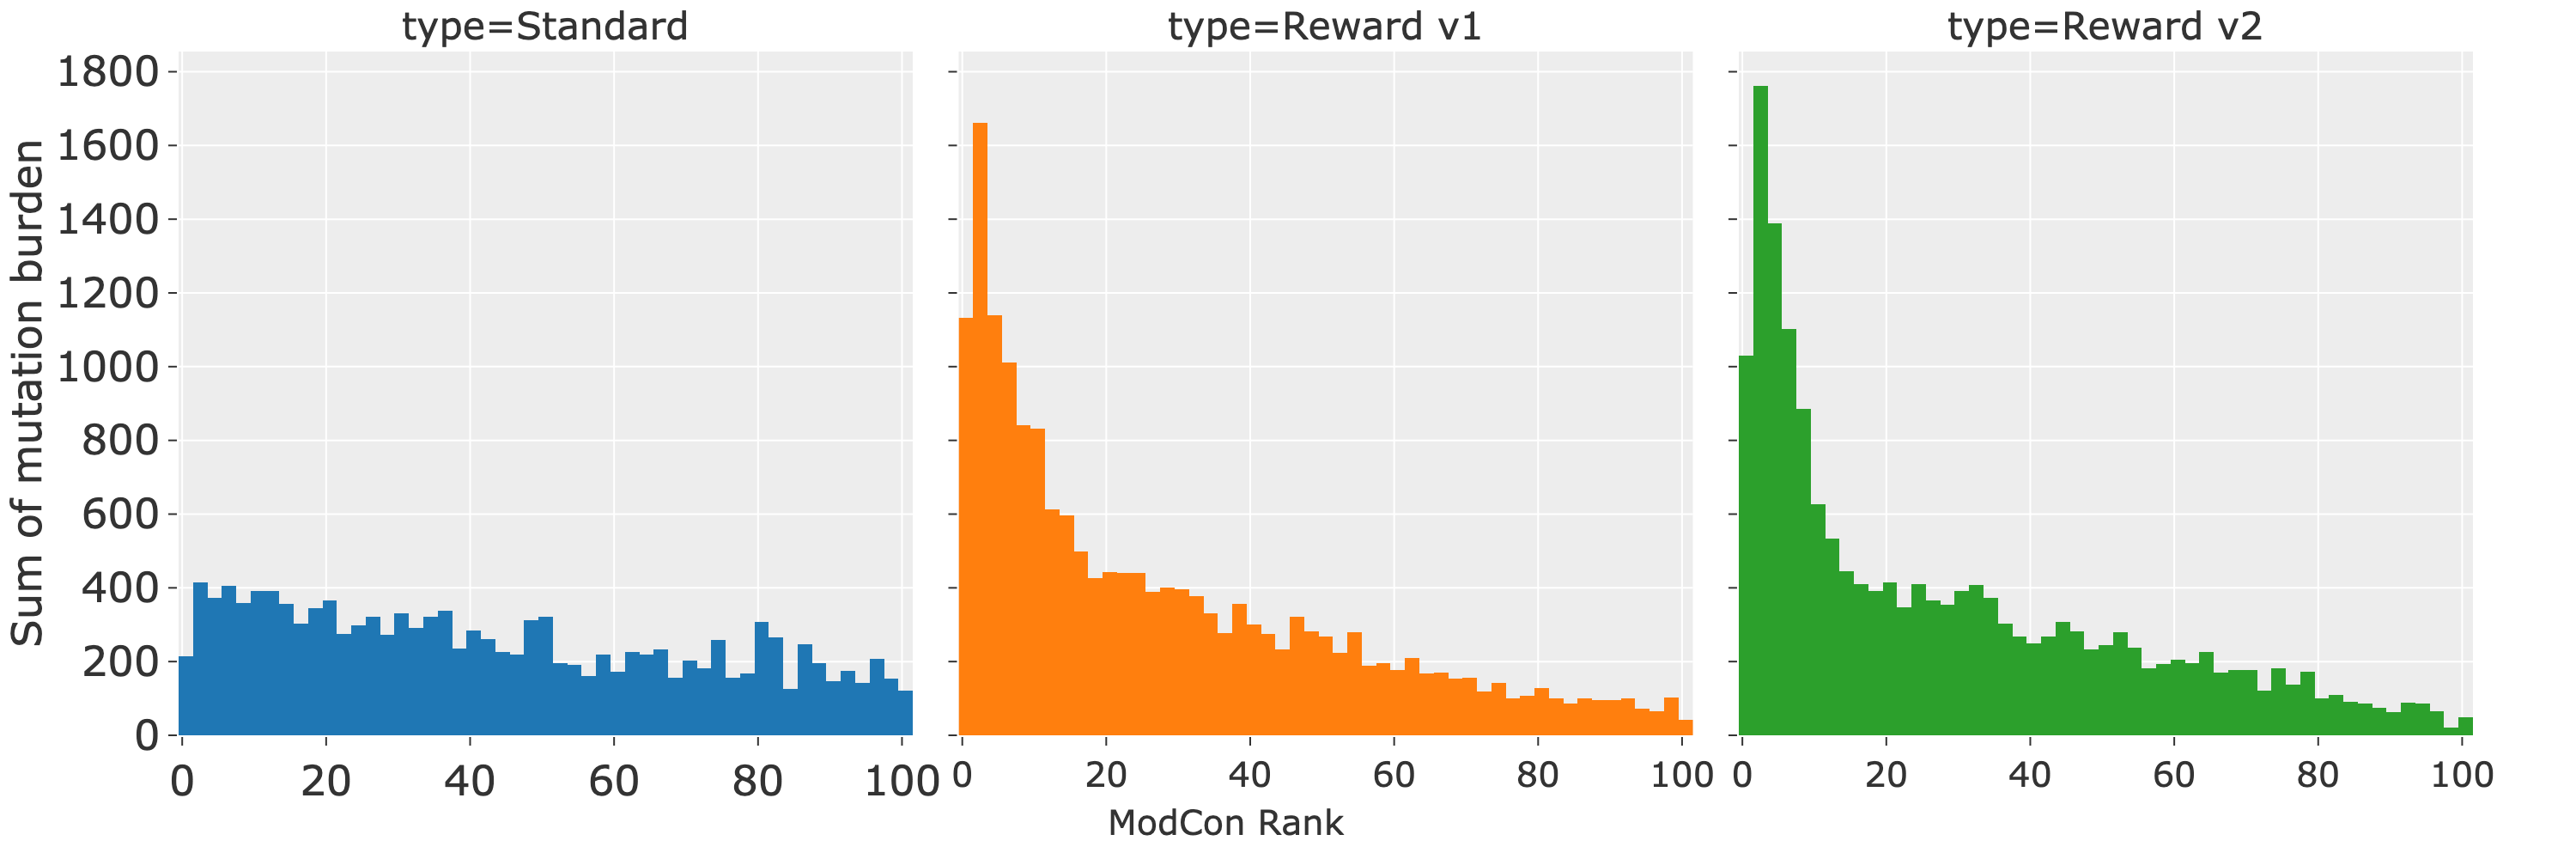
\includegraphics[width=1.0\textwidth,height=1.0\textheight,keepaspectratio]{Sections/Network_II/validation/tum_modCon_hist_3.png}
        \caption{Networks generated from the tumour dataset (TCGA)}
    \end{subfigure} %
    \begin{subfigure}{1.0\linewidth}
        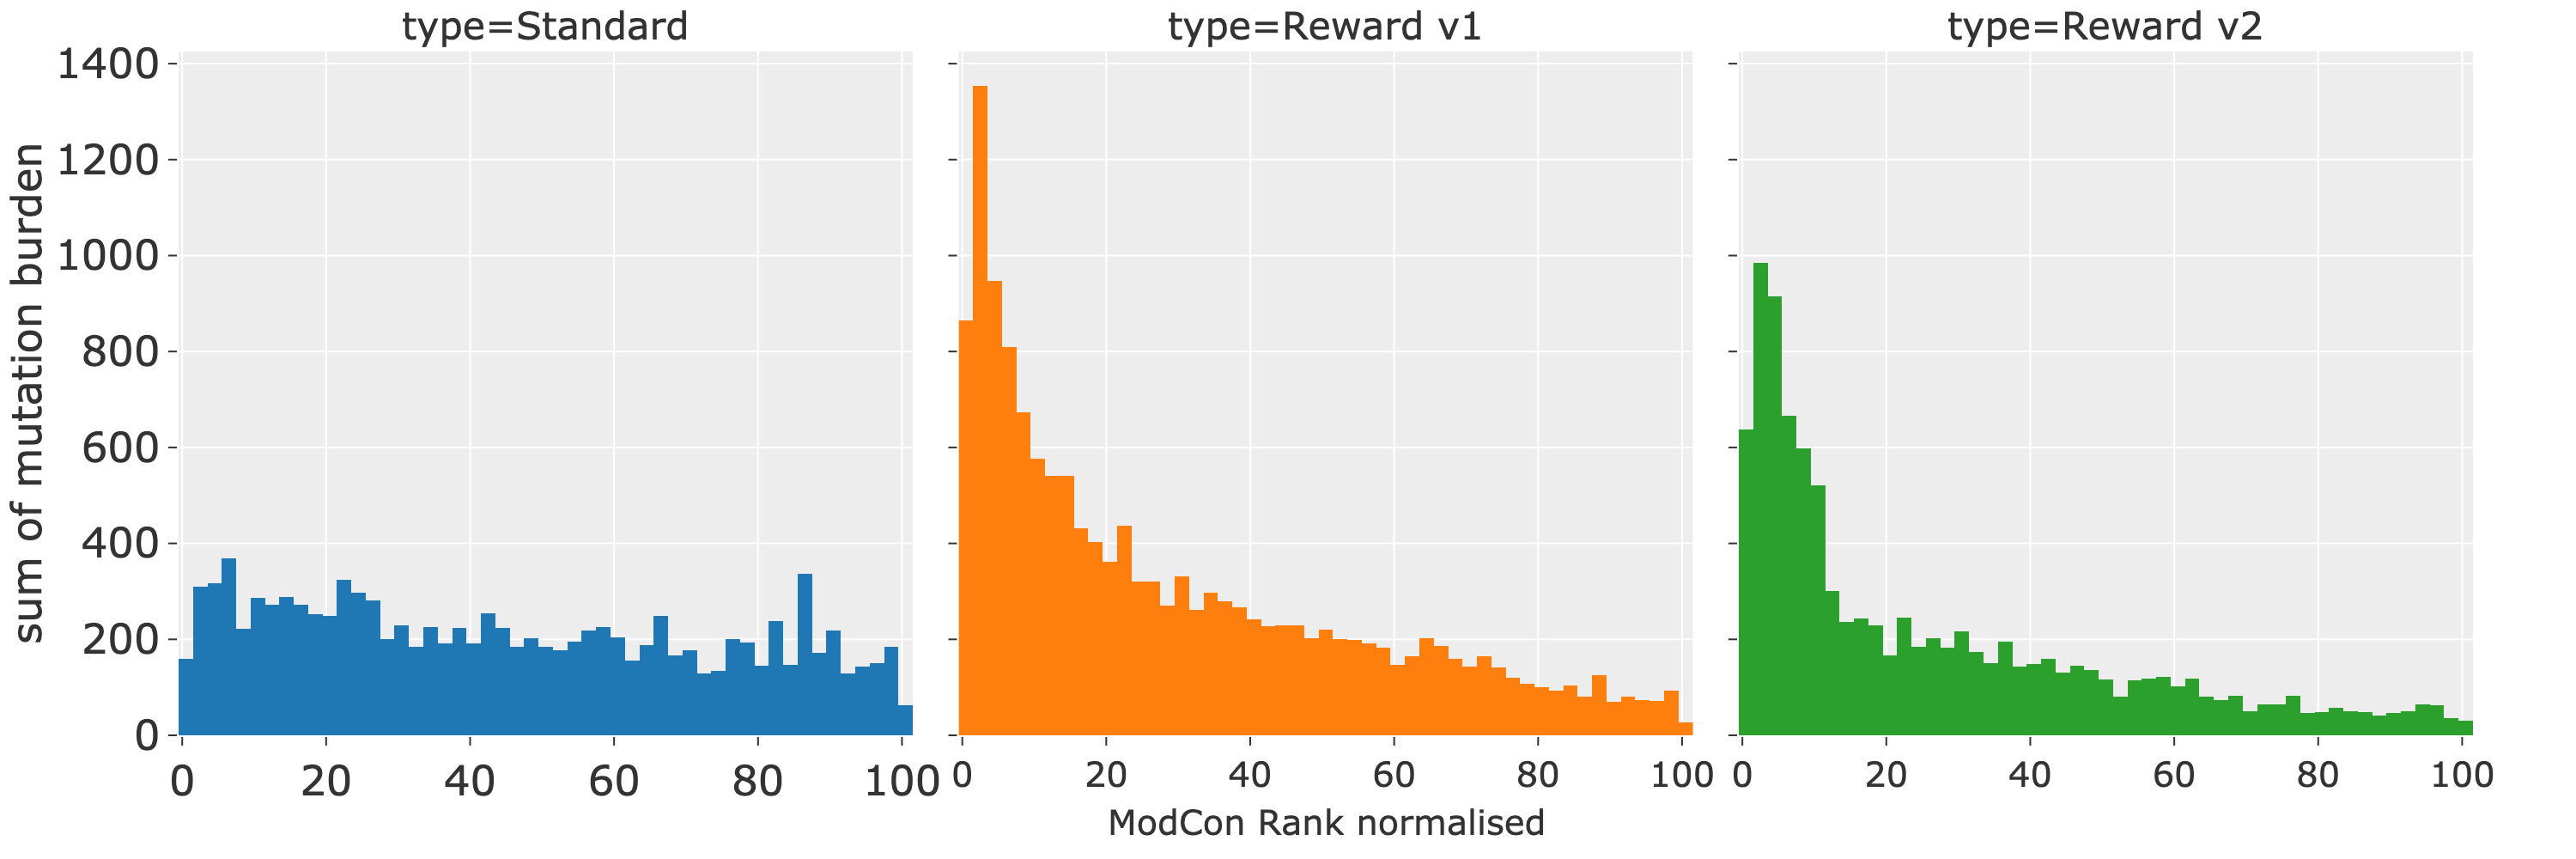
\includegraphics[width=1.0\textwidth, ,height=1.0\textheight,keepaspectratio]{Sections/Network_II/validation/non_tum_modCon_hist_3.png}
        \caption{Networks generated from the non-tumour dataset (JBU)}
    \end{subfigure}
    \caption[Mutation burden across the highest 100 ModCon]{The cumulative mutation burden from TCGA (Y-axis) over the ModCon Ranking (X-axis) for the three weight modifiers: Standard, Reward 1, and Reward 2 (sigmoid) across tumour and non-tumour datasets. The plot shows the sum of the mutation burden for the top 100 genes with the highest ModCon scores, which are used for MIBC clustering. While the two reward modifiers exhibit similar distributions in the tumour networks, they differ in the non-tumour graphs. This difference can be attributed to the community size imbalance and the fixed selection limit of 100 genes per community.}
    \label{fig:N_II:modCon_modifiers}
\end{figure}



\begin{table}[!htb]
  \centering
  \small
  \begin{tabularx}{\textwidth}{>{\hsize=.55\hsize}X|>{\hsize=.5\hsize}X|>{\hsize=.45\hsize}X}
    \toprule
    \textbf{Comparison} & \textbf{Mutation Burden} & \textbf{ModCon Rank} \\
    \midrule
    \multicolumn{3}{c}{\textbf{Tumour}} \\
    \midrule
    \textbf{Reward 1 vs Reward 2} & 9695120.0; $4.137e^{-12}$ & 9287455.0; 0.0012 \\
    \midrule
    \textbf{Standard vs Reward 1} & 6101149.5; $8.240e^{-8}$ & 7098464.5; $5.322e^{-9}$ \\
    \midrule
    \textbf{Standard vs Reward 2} & 7233820.5; 0.280 & 9287455.0; $2.249e^{-19}$ \\
    \midrule
    \multicolumn{3}{c}{\textbf{Non-tumour}} \\
    \midrule 
     \textbf{Reward 1 vs Reward 2} & 4752647.0; $3.03e^{-17}$ & 4418659.0; 0.0017 \\
    \midrule
    \textbf{Standard vs Reward 1} & 4653638.5; $3.04e^{-17}$ & 5804760.5; $7.07e^{-12}$ \\
    \midrule
    \textbf{Standard vs Reward 2} & 3782724.0; 0.314 & 4276523.5; $3.79e^{-21}$ \\
    \bottomrule
  \end{tabularx}
  \caption[Reward modifiers: Effect on Rank and Mutation Burden]{Compares the Mutation burden and ModCon Rank distributions between the three networks. The first value is represented by the result from the \acrlong{mw} while the second the p-value.}
  \label{tab:N_II:sig_mut_burden_rank}
\end{table}


% iMEV comparison
\subsection{MEV comparisons} \label{s:N_II:mev_comp}

Towards the last stages of the network pipeline, there is the MEV score, which bridges the gap between the gene to sample representation. This chapter introduced a new MEV score that integrates gene expression from both tumour and non-tumour as explained in \cref{s:N_II:iMEV}.

To validate the change in MEV, the non-tumour networks of $5,000$ genes, with $3$ genes per non-TF gene and $6$ for TF and hierarchical SBM was applied to determine the communities. The standard and Reward v2 networks were used for comparison. To be consistent with previous work, K-means with K=6 was used to contrast the subgroups by the two versions of the MEV. 

% The largest change occur across the subtypes found using the standard network, from where 
The results of the comparison are shown in \cref{fig:N_II:mevs_comp}, presenting the subtypes derived using the different MEVs scores, MEV\_1 (first iteration) and MEV\_2 (second iteration - integrative), in relation to previous classifications: the cluster analysis from \cref{s:clustering_analysis}, TCGA and consensus \citep{Robertson2017-mg,Kamoun2020-tj}. In the top comparison, where the subtypes derived from the standard networks, there is some change between the groups found using the two versions of the MEV scores.

The integrative MEV has a stronger effect on the MIBC subtyping in the reward-derived networks as seen in the bottom Sankey plot, where a subset of samples (n=20) that change from group 0 (Reward\_MEV\_1) to 2 (Reward\_MEV\_2) which has a considerable implication to the subtypes, where the largest group (0) becomes the only third group by size. The difference between the two MEVs was observed to increase as the number of groups for K-means increases, especially in the standard network; see \cref{fig:ap:mevs_comp} from the Appendix \cref{ap:N_II:val_mibc_comp}.  

This sub-section demonstrates that updating the MEV to integrate both tumour and non-tumour gene expressions has a limited impact on the MIBC subtypes. One possible reason for the smaller effect on the derived subgroups could be the lack of adjustment for community size imbalances. This is supported by the minimal changes observed in the reward network compared to the standard when K=7, as shown in \cref{fig:ap:mevs_comp}. The integrative MEV (iMEV) is preferred because it incorporates gene expression data from both datasets, while the previous versions treated the network merely as a complex gene selection mechanism.


\begin{figure}[!b]
    \centering
    \begin{subfigure}{1.0\linewidth}
        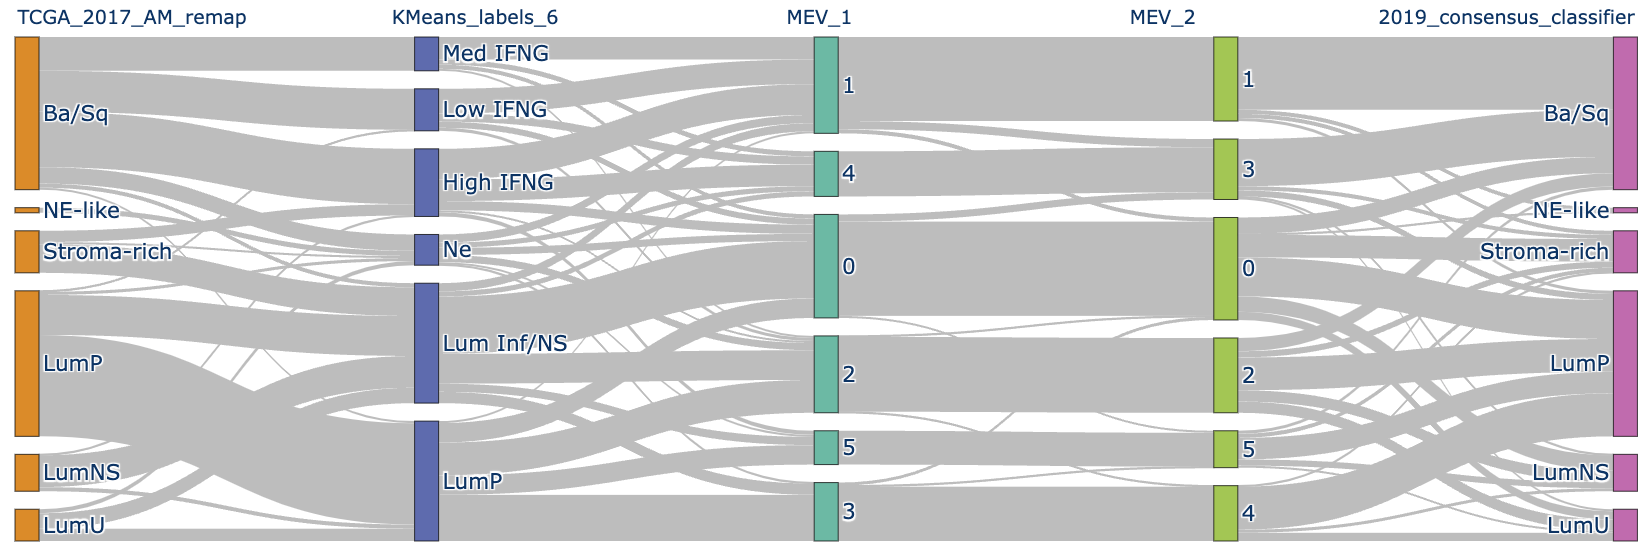
\includegraphics[width=1.0\textwidth,keepaspectratio]{Sections/Network_II/validation/mevs_comp_std.png}
        \caption{Standard networks}
    \end{subfigure} %
    \centering
    \begin{subfigure}{1.0\linewidth}
        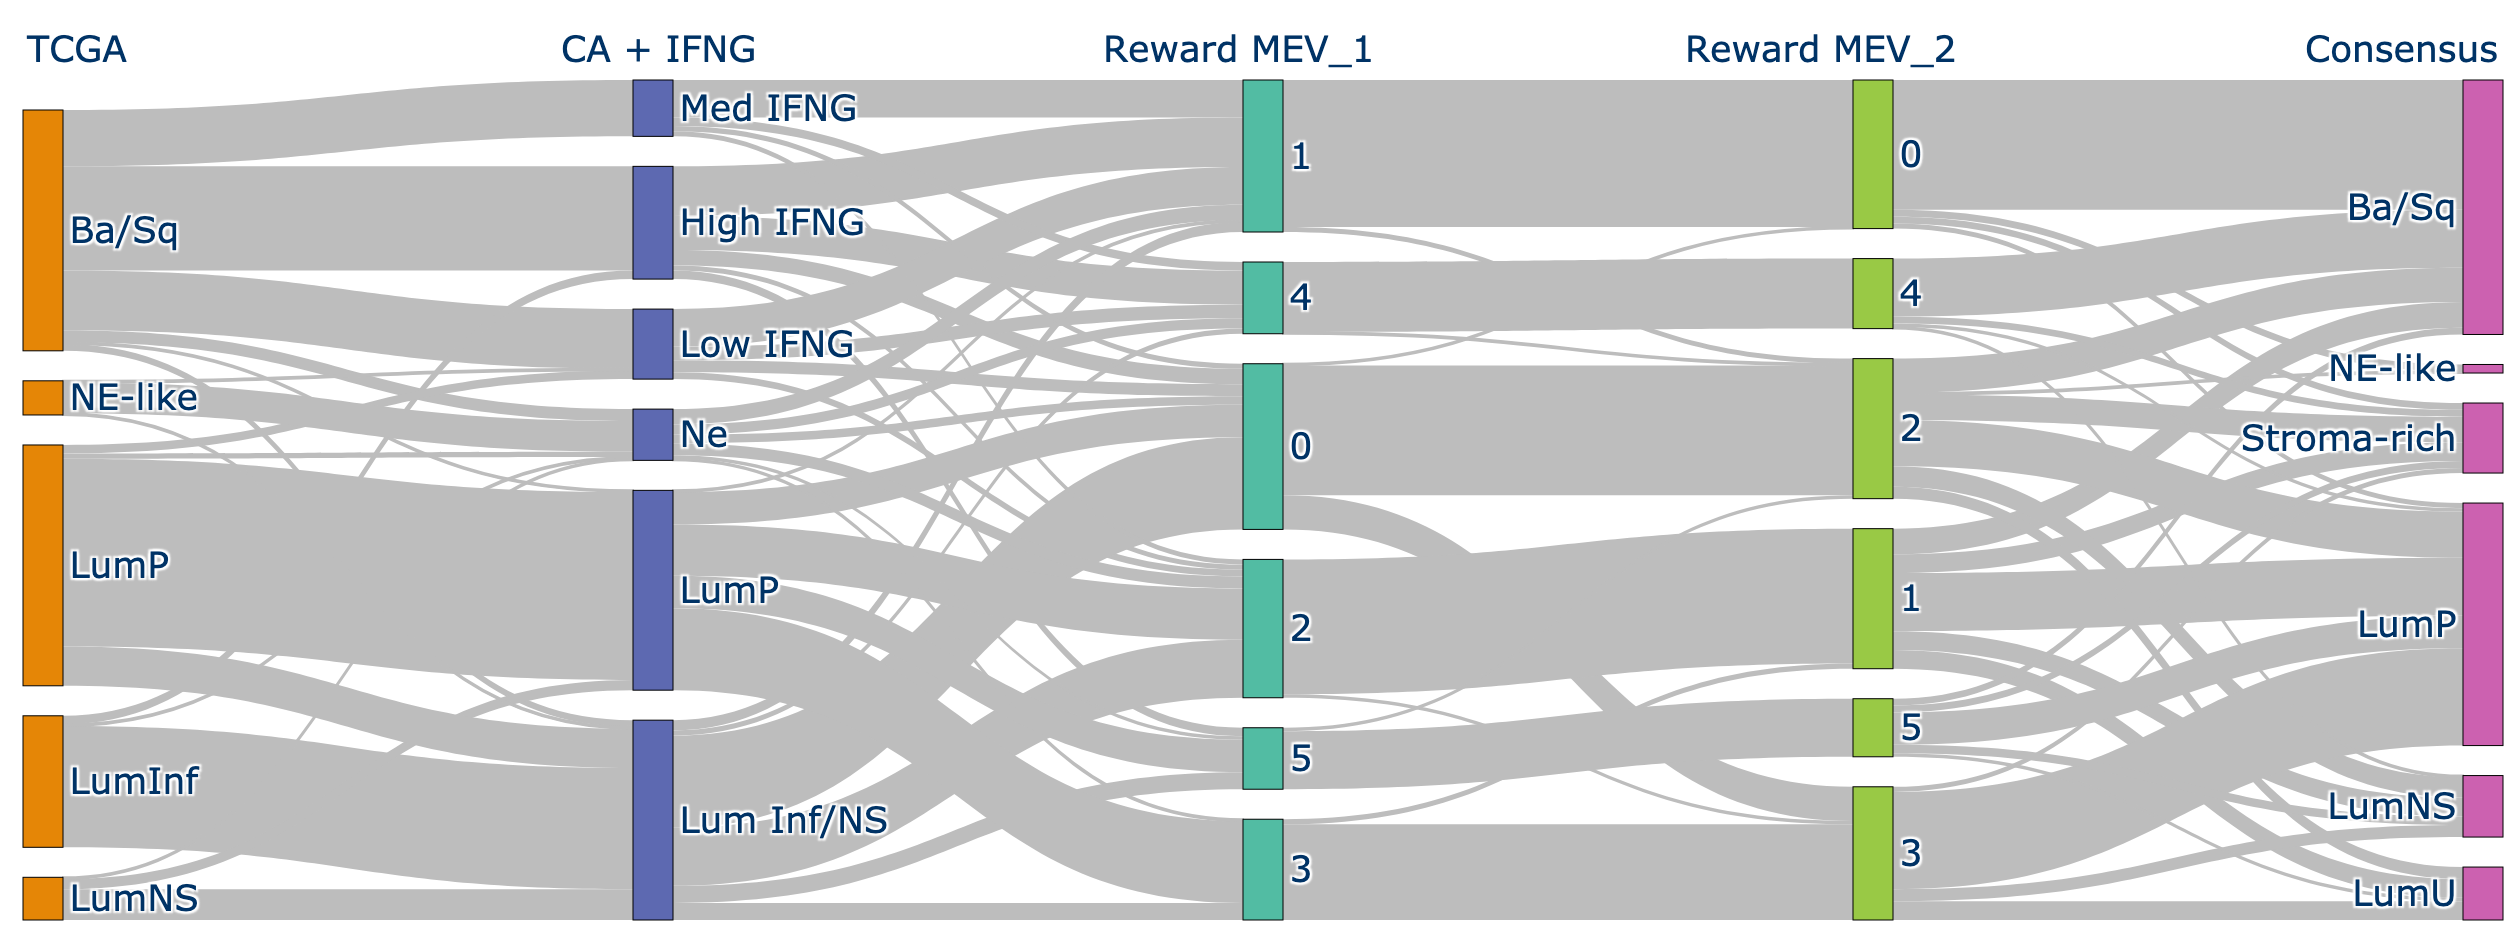
\includegraphics[width=1.0\textwidth,keepaspectratio]{Sections/Network_II/validation/mevs_comp_rwd.png}
        \caption{Reward v2 networks}
    \end{subfigure}
    \centering
    \caption[Subtypes derived from MEV vs iMEV]{In the two subfigures, sankey comparison between TCGA classification \citep{Robertson2017-mg}, the previous MIBC stratification from the cluster analysis in \cref{s:cs:bio_interp}, the two version of MEVs and the consensus \citep{Kamoun2020-tj}. The subtyping based on the two MEVs are the main groups to compare as the version of MEV only considers the gene expression from TCGA cohort while the second it integrates the non-tumour dataset as well; the other classifications are used for reference. There are a few samples changing between the groups derived using MEV\_1 and MEV\_2, showing that there new version of MEV has an effect on the subtypes, but smaller than expected. }
    \label{fig:N_II:mevs_comp}
\end{figure}




